


%% need no \usepackage{Sweave.sty}



%





%% use JSS class -- use 'nojss' to turn off header
\documentclass[shortnames,nojss,article]{jss}\usepackage{graphicx, color}
%% maxwidth is the original width if it is less than linewidth
%% otherwise use linewidth (to make sure the graphics do not exceed the margin)
\makeatletter
\def\maxwidth{ %
  \ifdim\Gin@nat@width>\linewidth
    \linewidth
  \else
    \Gin@nat@width
  \fi
}
\makeatother

\definecolor{fgcolor}{rgb}{0.2, 0.2, 0.2}
\newcommand{\hlnumber}[1]{\textcolor[rgb]{0,0,0}{#1}}%
\newcommand{\hlfunctioncall}[1]{\textcolor[rgb]{0.501960784313725,0,0.329411764705882}{\textbf{#1}}}%
\newcommand{\hlstring}[1]{\textcolor[rgb]{0.6,0.6,1}{#1}}%
\newcommand{\hlkeyword}[1]{\textcolor[rgb]{0,0,0}{\textbf{#1}}}%
\newcommand{\hlargument}[1]{\textcolor[rgb]{0.690196078431373,0.250980392156863,0.0196078431372549}{#1}}%
\newcommand{\hlcomment}[1]{\textcolor[rgb]{0.180392156862745,0.6,0.341176470588235}{#1}}%
\newcommand{\hlroxygencomment}[1]{\textcolor[rgb]{0.43921568627451,0.47843137254902,0.701960784313725}{#1}}%
\newcommand{\hlformalargs}[1]{\textcolor[rgb]{0.690196078431373,0.250980392156863,0.0196078431372549}{#1}}%
\newcommand{\hleqformalargs}[1]{\textcolor[rgb]{0.690196078431373,0.250980392156863,0.0196078431372549}{#1}}%
\newcommand{\hlassignement}[1]{\textcolor[rgb]{0,0,0}{\textbf{#1}}}%
\newcommand{\hlpackage}[1]{\textcolor[rgb]{0.588235294117647,0.709803921568627,0.145098039215686}{#1}}%
\newcommand{\hlslot}[1]{\textit{#1}}%
\newcommand{\hlsymbol}[1]{\textcolor[rgb]{0,0,0}{#1}}%
\newcommand{\hlprompt}[1]{\textcolor[rgb]{0.2,0.2,0.2}{#1}}%

\usepackage{framed}
\makeatletter
\newenvironment{kframe}{%
 \def\at@end@of@kframe{}%
 \ifinner\ifhmode%
  \def\at@end@of@kframe{\end{minipage}}%
  \begin{minipage}{\columnwidth}%
 \fi\fi%
 \def\FrameCommand##1{\hskip\@totalleftmargin \hskip-\fboxsep
 \colorbox{shadecolor}{##1}\hskip-\fboxsep
     % There is no \\@totalrightmargin, so:
     \hskip-\linewidth \hskip-\@totalleftmargin \hskip\columnwidth}%
 \MakeFramed {\advance\hsize-\width
   \@totalleftmargin\z@ \linewidth\hsize
   \@setminipage}}%
 {\par\unskip\endMakeFramed%
 \at@end@of@kframe}
\makeatother

\definecolor{shadecolor}{rgb}{.97, .97, .97}
\definecolor{messagecolor}{rgb}{0, 0, 0}
\definecolor{warningcolor}{rgb}{1, 0, 1}
\definecolor{errorcolor}{rgb}{1, 0, 0}
\newenvironment{knitrout}{}{} % an empty environment to be redefined in TeX

\usepackage{alltt}
\usepackage{booktabs,flafter,thumbpdf}
%\VignetteIndexEntry{An Introduction to dendextend}
%\VignetteKeywords{Dendrogram, hclust, heirarchical clustering, visualization, tanglegram, R}
%\VignettePackage{dendextend}
%\VignetteEngine{knitr::knitr}


\author{Tal Galili\\Tel-Aviv University \And Yoav Benjamini\\Tel-Aviv University}
\Plainauthor{Tal Galili, Yoav Benjamini}

\Plaintitle{dendextend: doing more with dendrogram objects in R}
\title{\pkg{dendextend}: doing more with\\ dendrogram objects in R}

\Abstract{
  The \pkg{dendextend} package extends the dendrogram objects in \proglang{R}.
}

\Keywords{Dendrogram, hclust, heirarchical clustering, visualization, tanglegram,  \proglang{R}}
\Plainkeywords{Dendrogram, hclust, heirarchical clustering, visualization, tanglegram, R}


% \Volume{40}
% \Issue{8}
% \Month{April}
% \Year{2011}
% \Submitdate{2010-11-15}
% \Acceptdate{2011-03-21}

\Address{
  Tal Galili \\
   Department of Statistics and Operations Research \\
   Tel Aviv University, Israel \\
   E-mail: \email{tal.galili@math.tau.ac.il}\\
   URLs: \url{http://www.r-statistics.com/}, 
         \url{http://www.r-bloggers.com/}\\

  Yoav Benjamini\\
   The Nathan and Lily Silver\\
   Professor of Applied Statistics\\
   Department of Statistics and Operations Research \\
   Tel Aviv University, Israel \\
   E-mail: \email{ybenja@tau.ac.il}\\
   URL: \url{http://www.tau.ac.il/~ybenja/}
}
\IfFileExists{upquote.sty}{\usepackage{upquote}}{}



\begin{document}

\vspace*{-0.25cm}

\section{Introduction}

\subsection{Introduction}


The \code{dendrogram} class provides general functions for handling tree-like structures in \proglang{R} \citep{R:Main}. It is intended as a replacement for similar functions in hierarchical clustering and classification/regression trees, such that all of these can use the same engine for plotting or cutting trees.

A dendrogram object represents a tree as a list object, with various attributes.

For example, let's create a dendrogram object based on an heirarchical clustering of 4 states in the U.S.:

\begin{knitrout}
\definecolor{shadecolor}{rgb}{0.969, 0.969, 0.969}\color{fgcolor}\begin{kframe}
\begin{alltt}
\hlcomment{# our data:}
\hlfunctioncall{data}(USArrests)
US_data <- USArrests[\hlfunctioncall{c}(2, 5, 32, 35), ]
\hlfunctioncall{print}(US_data)
\end{alltt}
\begin{verbatim}
##            Murder Assault UrbanPop Rape
## Alaska       10.0     263       48 44.5
## California    9.0     276       91 40.6
## New York     11.1     254       86 26.1
## Ohio          7.3     120       75 21.4
\end{verbatim}
\begin{alltt}

hc <- \hlfunctioncall{hclust}(\hlfunctioncall{dist}(US_data), \hlstring{"ave"})  # create an heirarchical clustering object
dend <- \hlfunctioncall{as.dendrogram}(hc)
\end{alltt}
\end{kframe}
\end{knitrout}




Dendrogram has several useful methods bundled with R:

\begin{knitrout}
\definecolor{shadecolor}{rgb}{0.969, 0.969, 0.969}\color{fgcolor}\begin{kframe}
\begin{alltt}
\hlfunctioncall{methods}(class = \hlstring{"dendrogram"})
\end{alltt}
\begin{verbatim}
##  [1] [[.dendrogram*         as.hclust.dendrogram* 
##  [3] cophenetic.dendrogram* cut.dendrogram*       
##  [5] head.dendrogram*       labels.dendrogram*    
##  [7] labels<-.dendrogram*   merge.dendrogram*     
##  [9] nleaves.dendrogram*    plot.dendrogram*      
## [11] print.dendrogram*      reorder.dendrogram*   
## [13] rev.dendrogram*        rotate.dendrogram*    
## [15] sort.dendrogram*       str.dendrogram*       
## [17] trim.dendrogram*       unroot.dendrogram*    
## 
##    Non-visible functions are asterisked
\end{verbatim}
\end{kframe}
\end{knitrout}



Here are some examples for their use:

\begin{knitrout}
\definecolor{shadecolor}{rgb}{0.969, 0.969, 0.969}\color{fgcolor}\begin{kframe}
\begin{alltt}
\hlfunctioncall{print}(dend)
\end{alltt}
\begin{verbatim}
## 'dendrogram' with 2 branches and 4 members total, at height 146.7
\end{verbatim}
\begin{alltt}
\hlfunctioncall{labels}(dend)
\end{alltt}
\begin{verbatim}
## [1] "Ohio"       "Alaska"     "California" "New York"
\end{verbatim}
\begin{alltt}
\hlfunctioncall{str}(dend)
\end{alltt}
\begin{verbatim}
## --[dendrogram w/ 2 branches and 4 members at h = 147]
##   |--leaf "Ohio" 
##   `--[dendrogram w/ 2 branches and 3 members at h = 44.1]
##      |--leaf "Alaska" 
##      `--[dendrogram w/ 2 branches and 2 members at h = 26.9]
##         |--leaf "California" 
##         `--leaf "New York"
\end{verbatim}
\begin{alltt}
\hlfunctioncall{str}(dend[[2]])  \hlcomment{# looking at one branch of the dendrogram}
\end{alltt}
\begin{verbatim}
## --[dendrogram w/ 2 branches and 3 members at h = 44.1]
##   |--leaf "Alaska" 
##   `--[dendrogram w/ 2 branches and 2 members at h = 26.9]
##      |--leaf "California" 
##      `--leaf "New York"
\end{verbatim}
\begin{alltt}
\hlfunctioncall{plot}(dend)
\end{alltt}
\end{kframe}

{\centering 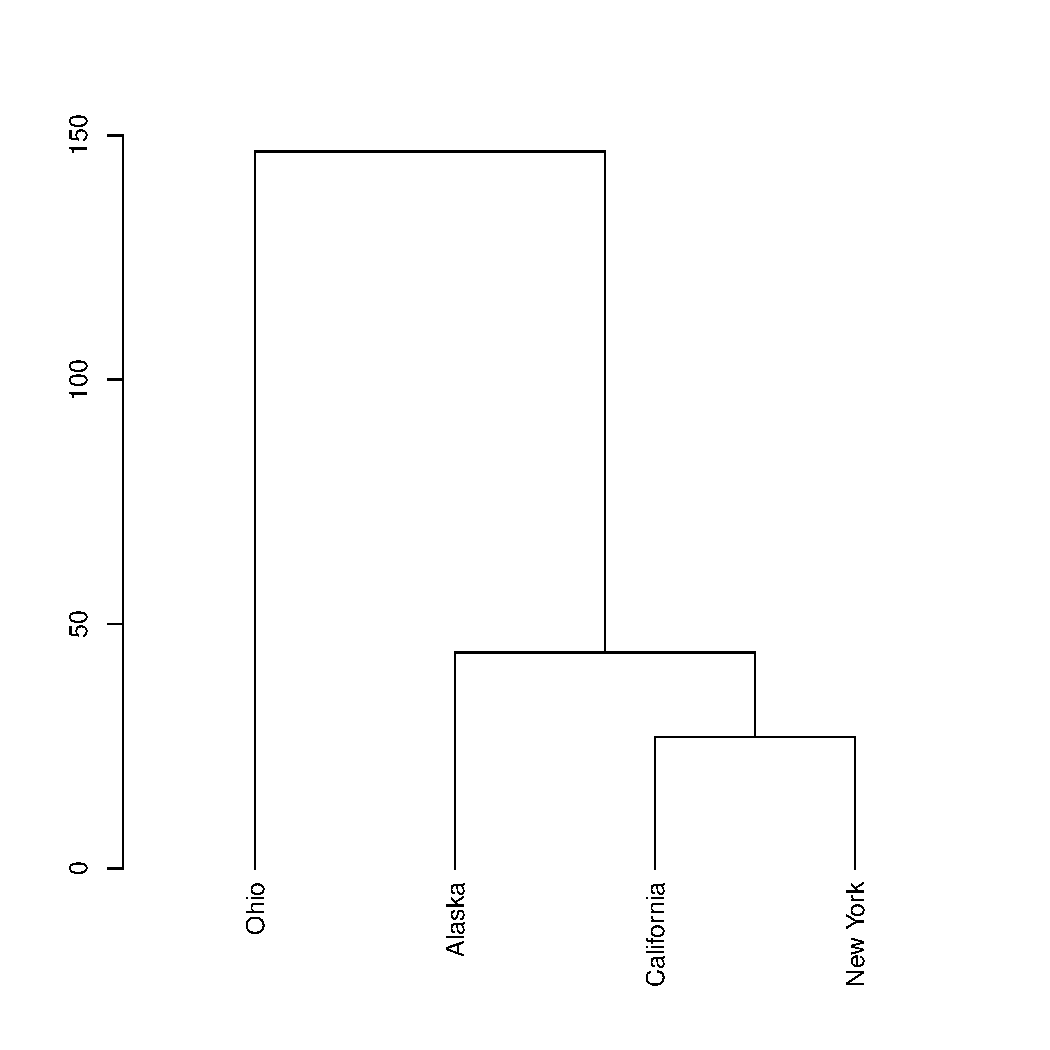
\includegraphics[width=4in,height=4in]{figure/unnamed-chunk-4} 

}



\end{knitrout}


You might notice how the order of the items (leaves/terminal nodes) of the dendrogram is different than their order in the table. In order to re-order the rows in the data-table to have the same order as the items in the dendrogram, we can use the \code{order.dendrogram} function:

\begin{knitrout}
\definecolor{shadecolor}{rgb}{0.969, 0.969, 0.969}\color{fgcolor}\begin{kframe}
\begin{alltt}
(new_order <- \hlfunctioncall{order.dendrogram}(dend))
\end{alltt}
\begin{verbatim}
## [1] 4 1 2 3
\end{verbatim}
\begin{alltt}
\hlcomment{# the order of the original items to have them be at the}
\hlcomment{# same order as they assume in the dendrogram}
\hlfunctioncall{print}(US_data[new_order, ])
\end{alltt}
\begin{verbatim}
##            Murder Assault UrbanPop Rape
## Ohio          7.3     120       75 21.4
## Alaska       10.0     263       48 44.5
## California    9.0     276       91 40.6
## New York     11.1     254       86 26.1
\end{verbatim}
\end{kframe}
\end{knitrout}



In order to see what our dendrogram (list) object includes, we need to use the \code{unclass} function, which will allow us to print the list as is, without going through the \code{print.dendrorgam} method:

\begin{knitrout}
\definecolor{shadecolor}{rgb}{0.969, 0.969, 0.969}\color{fgcolor}\begin{kframe}
\begin{alltt}
\hlfunctioncall{unclass}(dend)
\end{alltt}
\begin{verbatim}
## [[1]]
## [1] 4
## attr(,"members")
## [1] 1
## attr(,"height")
## [1] 0
## attr(,"label")
## [1] "Ohio"
## attr(,"leaf")
## [1] TRUE
## 
## [[2]]
## [[2]][[1]]
## [1] 1
## attr(,"members")
## [1] 1
## attr(,"height")
## [1] 0
## attr(,"label")
## [1] "Alaska"
## attr(,"leaf")
## [1] TRUE
## 
## [[2]][[2]]
## [[2]][[2]][[1]]
## [1] 2
## attr(,"label")
## [1] "California"
## attr(,"members")
## [1] 1
## attr(,"height")
## [1] 0
## attr(,"leaf")
## [1] TRUE
## 
## [[2]][[2]][[2]]
## [1] 3
## attr(,"label")
## [1] "New York"
## attr(,"members")
## [1] 1
## attr(,"height")
## [1] 0
## attr(,"leaf")
## [1] TRUE
## 
## attr(,"members")
## [1] 2
## attr(,"midpoint")
## [1] 0.5
## attr(,"height")
## [1] 26.9
## 
## attr(,"members")
## [1] 3
## attr(,"midpoint")
## [1] 0.75
## attr(,"height")
## [1] 44.14
## 
## attr(,"members")
## [1] 4
## attr(,"midpoint")
## [1] 0.875
## attr(,"height")
## [1] 146.7
\end{verbatim}
\end{kframe}
\end{knitrout}




We can see how each node in the dendrogram/list object has the following (self explaining) attributes:
Also, terminal nodes also has the "leaf" attribute (set to TRUE).
\begin{knitrout}
\definecolor{shadecolor}{rgb}{0.969, 0.969, 0.969}\color{fgcolor}\begin{kframe}
\begin{alltt}
\hlfunctioncall{names}(\hlfunctioncall{attributes}(dend)[-4])
\end{alltt}
\begin{verbatim}
## [1] "members"  "midpoint" "height"
\end{verbatim}
\end{kframe}
\end{knitrout}

Also, terminal nodes also has the "leaf" attribute (set to TRUE).

\subsection{Motivation for creating \code{dendextend}}



The \code{dendrogram} object has several \textbf{advantages}:

\begin{enumerate}
   \item \code{dendrogram} objects are simply list R objects. This makes their structure  very simple to understand by R users.
   \item \code{dendrogram} objects has various methods and functions for using them in R. 
   \item \code{dendrogram} objects are relatively simple to manipulte and extend.
   \item Other tree objects (such as *hclust*, and objects from the *{ape}* package) include an *as.dendrogram* method for converting their objects into a dendrogram.
\end{enumerate}


However, even with all of its advantages, the \code{dendrogram} class in R still lacks various basic features.

The \code{dendextend} package aims at filling some gaps in base R, by extending the available functions for dendrogram manipulation, statistical analysis, and visualization.

This vignettes Provides a step-by-step description of the functionality provided by the \code{dendextend} package.


\subsection{Installing \code{dendextend}}

To install the stable version from CRAN use:

\begin{knitrout}
\definecolor{shadecolor}{rgb}{0.969, 0.969, 0.969}\color{fgcolor}\begin{kframe}
\begin{alltt}
\hlfunctioncall{install.packages}(\hlstring{"dendextend"})  # not yet available from CRAN
\end{alltt}
\end{kframe}
\end{knitrout}



To install the \href{https://github.com/talgalili/dendextend}{GitHub version} use:

\begin{knitrout}
\definecolor{shadecolor}{rgb}{0.969, 0.969, 0.969}\color{fgcolor}\begin{kframe}
\begin{alltt}
\hlfunctioncall{if} (!\hlfunctioncall{require}(\hlstring{"devtools"})) \hlfunctioncall{install.packages}(\hlstring{"devtools"})
\hlfunctioncall{require}(\hlstring{"devtools"})
\hlfunctioncall{install_github}(\hlstring{"dendextend"}, \hlstring{"talgalili"})
\end{alltt}
\end{kframe}
\end{knitrout}



\section{Labels extraction and assignment}


\subsection{labels in base R}

In base R, the \code{labels} function is intended to find/extract a suitable set of labels from an object for use in printing or plotting, for example. By default, it uses the \code{names} and \code{dimnames} functions.

What base R \code{labels} function is mising is assignment. In the next few examples we will go through different examples of what the \code{dendextend} package offers for various objects.

\textbf{Credit:} These assignment functions were originally written by Gavin Simpson (in a post on \href{http://stackoverflow.com/questions/4614223/how-to-have-the-following-work-labelsx-some-value-r-question}{(stackoverflow)}), and adopted/adjusted to this package by Tal Galili.


\subsection{labels for vectors and matrixes}

In base R, for vectors, labels gives the \code{names} of the object. And if these are missing, then \code{labels} will give the vector itself as a character vector:

\begin{knitrout}
\definecolor{shadecolor}{rgb}{0.969, 0.969, 0.969}\color{fgcolor}\begin{kframe}
\begin{alltt}
x <- 1:3
\hlfunctioncall{names}(x)  \hlcomment{# this vector has no names}
\end{alltt}
\begin{verbatim}
## NULL
\end{verbatim}
\begin{alltt}
\hlfunctioncall{labels}(x)  \hlcomment{# this vector has no labels}
\end{alltt}
\begin{verbatim}
## [1] "1" "2" "3"
\end{verbatim}
\end{kframe}
\end{knitrout}


Assignment to names is available in base R and works as follows:

\begin{knitrout}
\definecolor{shadecolor}{rgb}{0.969, 0.969, 0.969}\color{fgcolor}\begin{kframe}
\begin{alltt}
x <- 1:3
\hlfunctioncall{names}(x) <- letters[1:3]  \hlcomment{# assignment for names is in base R}
\hlcomment{# both names and labels will give the same result:}
\hlfunctioncall{names}(x)
\end{alltt}
\begin{verbatim}
## [1] "a" "b" "c"
\end{verbatim}
\begin{alltt}
\hlfunctioncall{labels}(x)
\end{alltt}
\begin{verbatim}
## [1] "a" "b" "c"
\end{verbatim}
\end{kframe}
\end{knitrout}



The new labels assignment function will allow a user to change the labels of the vector just as if it was "names":

\begin{knitrout}
\definecolor{shadecolor}{rgb}{0.969, 0.969, 0.969}\color{fgcolor}\begin{kframe}
\begin{alltt}
x <- 1:3
\hlfunctioncall{labels}(x) <- letters[1:3]
\hlfunctioncall{names}(x)
\end{alltt}
\begin{verbatim}
## [1] "a" "b" "c"
\end{verbatim}
\begin{alltt}
\hlfunctioncall{labels}(x)
\end{alltt}
\begin{verbatim}
## [1] "a" "b" "c"
\end{verbatim}
\end{kframe}
\end{knitrout}


Labels assignment are also available for matrixes.


\subsection{labels for dendrogram objects}

\subsection{labels for hclust objects}




% 
% 
% a short review of other approaches and give some historical
% background on the development of \pkg{dendextend}.
% 
% 
% Several examples are included to illustrate the functionality of \pkg{dendextend}. Many more examples are available within
% the package. % , both as explicit examples and as part of the numerous unit tests.
% %
% The \pkg{dendextend} package is available from the Comprehensive \proglang{R} Archive Network (CRAN)
% at \url{http://CRAN.R-project.org/package=dendextend}.
% 
% \makeatletter
% \if@nojss
%   This vignette will one day corresponds to a paper 
%   
% %   published in the \textsl{Journal of Statistical Software}. It is currently still identical to the published paper.  
%   
%   Over time, this vignette version may receive minor
%   updates. For citations, please use %the \cite{JSS:dendextend} or
%   % \cite{Eddelbuettel:2013:dendextend}; details are also provided in
%   \proglang{R} via \texttt{citation("dendextend")}.
% 
%   This version corresponds to \pkg{dendextend} version dendextend.version and was typeset on now.date.
% \fi
% \makeatother
% 

% \subsection{Historical context}
% \subsection{Related work}

%%% \cite - name and date in (),, \citep - (all in ())
% \cite{TempleLang:2009:RGCCTranslationUnit}, 

% \subsection[dendextend use cases]{\pkg{dendextend} use cases}
% \label{sec:classic_dendextend}

% \subsection[dendextend class hierarchy]{\pkg{dendextend} class hierarchy}
% \subsection{Derived classes}

% \subsection{Character vectors}

% \section[R and C++ data interchange]{\proglang{R} and \proglang{C++} data interchange}

% \subsection[C++ to R: wrap]{\proglang{C++} to \proglang{R}: \code{wrap}}
% \subsection[R to C++: as]{\proglang{R} to \proglang{C++}: \code{as}}

% The \citep command is used where the author name is to appear inside the parentheses alongside the date.
% \citep{Sanderson:2010:Armadillo}.


% \subsection{Implicit use of converters}

% \section{Function calls}
% \label{sec:functions}

% \section{Using code `inline'}
% \label{sec:inline}
% \code{update.packages()} 
% \footnote{This presumes a platform for which pre-built binaries are}
% \cite{CRAN:dendextend:Attributes} for more details.

% \section{Using Standard Template Library algorithms}

% \citep{Plauger+Et+Al:2000:STL}. 


% \section{Error handling}
% \subsection[C++ exceptions in R]{\proglang{C++} exceptions in \proglang{R}}
% \subsection[R errors in C++]{\proglang{R} errors in \proglang{C++}}


% \section{Performance comparison}
% \label{sec:perfcomp}



% %
% \begin{Code}
% ...
% \end{Code}
% %

% are summarized in Table~\ref{tab:benchmark} below.
% 
% \begin{table}[t]
%   \begin{center}
%     \begin{small}
%       \begin{tabular}{lrr}
%         \toprule
%         Implementation                    & Time in millisec. & Relative to \proglang{R} API \\
%         \cmidrule(r){2-3}
%         \proglang{R} API (as benchmark)             &  218       & \\
%         \pkg{dendextend} sugar                        &  145       & 0.67 \\
%         \code{NumericVector::iterator}    &  217       & 1.00 \\
%         \code{NumericVector::operator[]}  &  282       & 1.29 \\
%         %\code{dendextendVector<double>}         &  683       & 3.13 \\
%         \bottomrule
%       \end{tabular}
%     \end{small}
%     \caption{Run-time performance of the different convolution examples.}
%     \label{tab:benchmark}
%   \end{center}
% \end{table}
% 

% \section{On-going development}
% \label{sec:ongoing}

% \code{head},


\section{Summary}

The \pkg{dendextend} package presented in this paper greatly extends the available functionality of the dendrogram objects in \proglang{R}.

% compiled \proglang{C++} code with \proglang{R}.
% \pkg{dendextend} provides a \proglang{C++} class hierarchy which allows manipulation of \proglang{R} data structures in \proglang{C++}
% using member functions and operators directly related to the type
% of object being used, thereby reducing the level of expertise
% required to master the various functions and macros offered by the
% internal \proglang{R} API. The classes assume the entire
% responsibility of garbage collection of objects, relieving the
% programmer from book-keeping operations with the protection stack
% and enabling him/her to focus on the underlying problem.
% 
% Data interchange between \proglang{R} and \proglang{C++} code is performed by the \code{wrap()} and
% \code{as()} template functions. They allow the programmer to write logic in terms
% of \proglang{C++} data structures, and facilitate use of modern libraries such as the
% Standard Template Library (STL) and its containers and algorithms. The
% \code{wrap()} and \code{as()} template functions are extensible by
% design. They are also used either explicitly or implicitly throughout the API.
% By using only thin wrappers around \code{SEXP} objects and adopting \proglang{C++}
% idioms such as iterators, the footprint of the \pkg{dendextend} API
% is very lightweight, and does not incur a significant performance penalty.
% 
% The \pkg{dendextend} API offers opportunities to dramatically reduce the complexity
% of code, which should lower the initial cost of writing code and improve code readability, maintainability, and
% reuse---without incurring noticeable penalties in run-time performance.



% \section*{Acknowledgments}
% 
% Detailed comments and suggestions by editors as well as anonymous referees
% are gratefully acknowledged.  We are also thankful for code contributions by
% Douglas Bates and John Chambers, as well as for very helpful suggestions by Uwe
% Ligges, Brian Ripley and Simon Urbanek concerning the build systems for different
% platforms.   Last but not least, several users provided very fruitful
% ideas for new or extended features via the \code{dendextend-devel} mailing list.


\bibliography{dendextend-tutorial}

\vspace*{-0.35cm}

\end{document}

%%% Local Variables:
%%% mode: latex
%%% TeX-master: t
%%% End:


%% library(knitr)
%% Sweave2knitr('vignettes\\dendextend-tutorial.rnw')
